\documentclass[aspectratio=169,11pt]{beamer}
\usetheme[progressbar=frametitle,numbering=fraction,sectionpage=none]{metropolis}
\metroset{block=transparent}
\usepackage{amsmath,amssymb,booktabs,tabularx,array,ragged2e,tikz}
\usetikzlibrary{arrows.meta,positioning}
\definecolor{SoftBlue}{RGB}{76,112,150}
\definecolor{BlockBlue}{RGB}{228,236,246}
\definecolor{BlockBlueDark}{RGB}{207,222,239}
\definecolor{SoftGreen}{RGB}{34,110,91}
\definecolor{Accent}{RGB}{169,83,37}
\definecolor{Ink}{RGB}{32,40,52}
\definecolor{Secondary}{RGB}{73,88,104}
\setbeamercolor{normal text}{fg=Ink,bg=white}
\setbeamercolor{structure}{fg=SoftBlue}
\setbeamercolor{frametitle}{fg=Ink,bg=white}
\setbeamercolor{progress bar}{fg=SoftBlue,bg=gray!20}
\setbeamercolor{alerted text}{fg=SoftBlue}
\setbeamercolor{title separator}{fg=SoftBlue}
\setbeamercolor{block title}{fg=Ink,bg=BlockBlueDark}
\setbeamercolor{block body}{fg=Ink,bg=BlockBlue}
\setbeamertemplate{navigation symbols}{}
\AtBeginEnvironment{frame}{\setlength{\parskip}{2pt}\raggedright}
\setbeamersize{text margin left=7mm,text margin right=7mm}
\setbeamerfont{frametitle}{size=\large,series=\bfseries}
\newcolumntype{Y}{>{\RaggedRight\arraybackslash}X}
\newcommand{\kterm}[1]{{\color{SoftBlue}\bfseries #1}}
\newcommand{\lead}[1]{\par{\bfseries\color{SoftBlue}#1}\par}
\newcommand{\notefoot}[1]{\par\vfill{\fontsize{8}{9.3}\selectfont\color{Secondary}#1\par}}
\newcommand{\signal}[1]{\par\smallskip{\color{SoftGreen}\bfseries #1}\par}
\newcommand{\tinyhead}[1]{{\color{Secondary}\footnotesize\bfseries #1}}
\tikzset{edge/.style={-{Stealth},draw=SoftBlue,very thick}, panel/.style={draw=SoftBlue!50,fill=BlockBlue,rounded corners=3pt,align=center,minimum height=.9cm,inner sep=3pt}, norm/.style={draw=SoftBlue,line width=1pt}, fillzone/.style={fill=SoftBlue!23,draw=SoftBlue,line width=.9pt}}
\newcommand{\hint}[1]{{\color{Secondary}\footnotesize #1}}
\newcommand{\paired}[2]{\begin{columns}[T,onlytextwidth]\begin{column}{.48\linewidth}#1\end{column}\begin{column}{.48\linewidth}#2\end{column}\end{columns}}
\title{Taylor-Model Reachability for Neural-Network-Controlled Systems}
\hypersetup{pdftitle={Taylor-Model Reachability for Neural-Network-Controlled Systems},pdfauthor={Research presentation}}
\begin{document}

\begin{frame}[plain]
\vfill
{\raggedright\LARGE\bfseries Taylor-Model Reachability\\for Neural-Network-Controlled Systems\par}
\smallskip
{\color{SoftBlue}\rule{\linewidth}{.9pt}}\par
\vfill
\end{frame}

\begin{frame}{One control action carries uncertainty into the next state}
\small
At a controller update, a possible state has the form \(x=P(r)+e\). The parameter \(r\) selects a point in the starting set. The polynomial \(P\) tracks its influence, and \(e\) ranges over an interval of remaining error.
\begin{center}
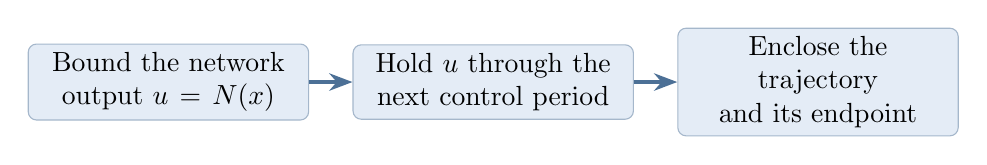
\begin{tikzpicture}
\node[panel,text width=3.35cm](a){Bound the network\\output \(u=N(x)\)};
\node[panel,text width=3.35cm,right=.55cm of a](b){Hold \(u\) through the\\next control period};
\node[panel,text width=3.35cm,right=.55cm of b](c){Enclose the trajectory\\and its endpoint};
\draw[edge](a)--(b);\draw[edge](b)--(c);
\end{tikzpicture}
\end{center}
Both methods keep a control polynomial and a remainder. We changed how that remainder is formed and tightened, how a local integration error can be validated, and how earlier errors are transported.
\notefoot{Huan denotes the implementation used in our experiments. His manuscript also describes additional strict arithmetic and controller bounds.}
\end{frame}

\begin{frame}{A rounded coefficient changes the stored control}
\small
Let \(N(x)=0.25x\), \(x=0.27r\), and \(r\in[-1,1]\). Store coefficients to two decimal places.\par
\paired{\lead{Terms in Huan's injection}
The incoming state error and the controller certificate gap are both zero.
\[
 V(r)=0.07r\quad\text{is stored.}
\]}{\lead{Extra term in our strict injection}
The exact coefficient is \(0.25\times0.27=0.0675\). Relative to the stored polynomial, the discrepancy is
\[
 N(x)-V(r)=-0.0025r.
\]
Its range is \([-0.0025,0.0025]\).}
\signal{We add a bound for this coefficient error to the control remainder.}
\notefoot{Huan also describes strict rounding compensation in his manuscript. Outward arithmetic can enlarge the exact discrepancy shown.}
\end{frame}

\begin{frame}{One slope, two ways to bound the controller residual}
\small
Take \(N(x)=\max(0,x)\) for \(-1\le x\le1\) and fix the slope at one. The residual is \(g(x)=N(x)-x\). Suppose the original certificate says \(-1\le g(x)\le1.5\).\par\medskip
\paired{\lead{Huan injects the supplied certificate}
The interval \([-1,1.5]\) has center \(0.25\) and radius \(1.25\). Written as a polynomial and centered remainder, the resulting enclosure is
\[
 N(x)\in (x+0.25)+[-1.25,1.25].
\]}{\lead{We evaluate the residual again}
For \(x\in[-1,0]\), \(g(x)=-x\in[0,1]\). For \(x\in[0,1]\), \(g(x)=0\). Both pieces together require only \([0,1]\).
\[
 N(x)\in (x+0.5)+[-0.5,0.5].
\]}
\signal{The slope stays at one. The independent check reduces the residual width from 2.5 to 1 and moves the center.}
\notefoot{Both paths receive the same illustrative loose certificate.}
\end{frame}

\begin{frame}{Why the order of combination matters}
\small
\paired{\lead{Different inputs require a hull}
At \(x=-1\), the residual equals one. At \(x=1\), it equals zero. The hull of \([0,1]\) and \(\{0\}\) retains both possibilities.
\par\smallskip
Intersecting those two images would lose the valid value at \(x=-1\).}{\lead{Two bounds on one input domain}
On each piece our module computes a forward bound and a bound that delays boxing activation errors. Both enclose the same residual on that piece, so we intersect them.}
\begin{block}{What delaying one error can preserve}
One shared activation error \(\eta\in[-0.1,0.1]\) reaches an output along two paths. Adding their coefficients gives \((3-3)\eta=0\). Boxing the paths separately gives \([-0.3,0.3]+[-0.3,0.3]=[-0.6,0.6]\).
\end{block}
\notefoot{This example explains the added evaluator. The tested implementation accepts rectified networks with four inputs, two hidden layers of 25 neurons and two outputs.}
\end{frame}

\begin{frame}{A second certificate keeps the entire polynomial fixed}
\small
Use the same controller \(N(x)=\max(0,x)\). This time the stored polynomial is \(V(x)=x/2\). Give both paths the valid starting enclosure \(N(x)-V(x)\in[-0.5,1]\).
\par\smallskip
\paired{\lead{Huan's benchmark path}
The next operation receives \(V\) and its original remainder \([-0.5,1]\). }
{\lead{Our additional anchor check}
A second certificate gives \(x/2\le N(x)\le x/2+0.5\). Subtract the same \(V\) throughout, then intersect
\[
 [-0.5,1]\cap[0,0.5]=[0,0.5].
\]}
\begin{block}{Check the two endpoints and the middle}
The discrepancy \(N(x)-x/2=|x|/2\) is 0.5 at both endpoints and zero at the middle. All coefficients stay fixed.
\end{block}
\notefoot{The first bound is illustrative. Quadrotor used 50 additional certificates, one per controller update.}
\end{frame}

\begin{frame}{What the tighter control changes in one plant step}
\small
At input \(x=0.6\), the polynomial gives \(V=0.3\) and the true held control is \(u=0.6\). Start a plant at \(y(0)=0\) with \(y'=u\). After 0.1 seconds, \(y=0.1u\).
\par\smallskip
\renewcommand{\arraystretch}{1.18}
\noindent\begin{tabularx}{\dimexpr\linewidth-1pt\relax}{@{}Yccc@{}}\toprule
& Control enclosure & Endpoint enclosure & Width\\\midrule
First remainder & \(0.3+[-0.5,1]\) & \([-0.02,0.13]\) & 0.15\\
Anchored remainder & \(0.3+[0,0.5]\) & \([0.03,0.08]\) & 0.05\\\bottomrule
\end{tabularx}\par
\begin{center}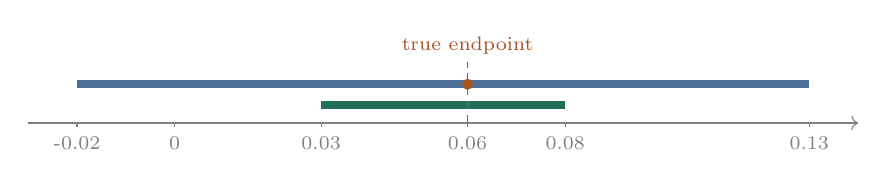
\begin{tikzpicture}[x=.62cm,y=.41cm,font=\scriptsize]
\draw[->,gray](-3,0)--(14,0);
\foreach \x/\lab in {-2/-0.02,0/0,3/0.03,6/0.06,8/0.08,13/0.13}{\draw[gray](\x,0)--++(0,-.14)node[below]{\lab};}
\draw[SoftBlue,line width=2.8pt](-2,1.2)--(13,1.2);
\draw[SoftGreen,line width=2.8pt](3,.55)--(8,.55);
\draw[Accent,densely dashed](6,0)--(6,1.9);\fill[Accent](6,1.2)circle(2pt);
\node[anchor=south,text=Accent] at(6,1.83){true endpoint};
\end{tikzpicture}\end{center}
\notefoot{Both estimates enclose the true endpoint 0.06.}
\end{frame}

\begin{frame}{Two shapes for the same local error budget}
\small
Consider \(y'=y\), \(y(0)=1\), step length \(h=0.1\), and candidate polynomial \(Q(\tau)=1+\tau\). Local time \(\tau\) runs from zero to \(h\). Both checks use the same proposed endpoint error interval \(R=[-0.0055,0.0055]\).
\par\medskip
\paired{\lead{Huan's ordinary inclusion check}
\centering\(y(\tau)-Q(\tau)\in R\)\par
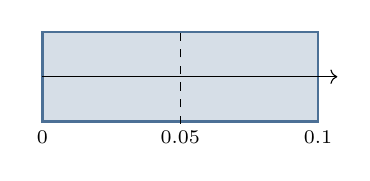
\begin{tikzpicture}[x=.7cm,y=.57cm]\filldraw[fillzone](0,-1)rectangle(5,1);\draw[->](0,0)--(5.35,0);\draw[dashed](2.5,-1.05)--(2.5,1.08);\node[below,font=\scriptsize] at(0,-1){0};\node[below,font=\scriptsize] at(2.5,-1){0.05};\node[below,font=\scriptsize] at(5,-1){0.1};\end{tikzpicture}\par
At half a step, \(\pm0.0055\).}
{\lead{Our time-weighted inclusion check}
\centering\(y(\tau)-Q(\tau)\in (\tau/h)R\)\par
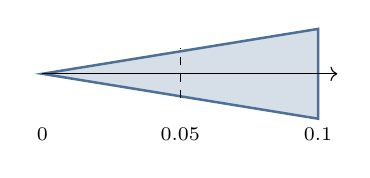
\begin{tikzpicture}[x=.7cm,y=.57cm]\filldraw[fillzone](0,0)--(5,1)--(5,-1)--cycle;\draw[->](0,0)--(5.35,0);\draw[dashed](2.5,-.55)--(2.5,.58);\node[below,font=\scriptsize] at(0,-1){0};\node[below,font=\scriptsize] at(2.5,-1){0.05};\node[below,font=\scriptsize] at(5,-1){0.1};\end{tikzpicture}\par
At half a step, \(\pm0.00275\).}
\notefoot{The weighted shape starts at zero because the candidate matches its local seed. With uncertain initial states, the seed still represents their full range.}
\end{frame}

\begin{frame}{The same candidate fails one check and passes the other}
\small
For an allowed error \(e(s)\), the integral equation gives a new discrepancy
\[
 D(\tau)=1+\int_0^\tau(1+s+e(s))\,ds-(1+\tau)
         =\tau^2/2+\int_0^\tau e(s)\,ds .
\]
\paired{\lead{Constant error allowance}
With \(e(s)\in R\), \(D(\tau)\in\tau^2/2+\tau R\). Over the step, this gives
\[
 [-0.00055,\mathbf{0.00555}].
\]
The upper end exceeds \(0.0055\).}
{\lead{Time-weighted error allowance}
With \(e(s)\in(s/h)R\), the normalized discrepancy lies in \(h\tau/2+(\tau/2)R\). Over the step, this gives
\[
 [-0.000275,\mathbf{0.005275}].
\]
Both ends fit inside \(R\).}
\notefoot{For the weighted test, integrate first to get \(D(\tau)\in\tau^2/2+\tau^2R/(2h)\), then cancel the common time factor. The normalized expression extends continuously to zero.}
\end{frame}

\begin{frame}{How earlier errors reach the present}
\small
Both methods carry old remainder increments through later linear maps. Take one old increment in \([0,3]\) and an exact transport factor of \(1/3\). The exact transported interval is \([0,1]\).\par\smallskip
\renewcommand{\arraystretch}{1.25}
\noindent\begin{tabularx}{\dimexpr\linewidth-1pt\relax}{@{}>{\RaggedRight\arraybackslash}p{3.0cm}Y@{}}\toprule
Representation & Two-decimal illustration\\\midrule
Huan's point products & The point product before compensation gives \(0.33[0,3]=[0,0.99]\). The factor discrepancy contributes \((1/3-0.33)[0,3]=[0,0.01]\). Adding it separately encloses \([0,1]\).\\
Our interval products & Store the factor as \([0.33,0.34]\). Multiplication gives \([0.33,0.34][0,3]=[0,1.02]\), including the exact upper endpoint.\\\bottomrule
\end{tabularx}\par
\notefoot{The separate compensation illustrates an option in Huan's manuscript. Our strict path encloses the normalized endpoint factors and their products directly. Carrying intervals can cost time and enlarge a bound.}
\end{frame}

\begin{frame}{What actually ran on the less-robust Double Pendulum}
\small
We bounded the same controller for 225 initial boxes over 20 control updates. The added residual evaluator split each four-dimensional controller box into four pieces along each coordinate.
\[
 \underbrace{4^4}_{256\ \mathrm{subboxes\ per\ box}}
 \qquad
 \underbrace{225\times256\times20}_{1{,}152{,}000\ \mathrm{subbox\ evaluations}} .
\]
\paired{\lead{Controller work}
The network verifier supplied 20 original bound calls. Our evaluator processed the subboxes in batches, using the slope already returned for each box.}{\lead{Integration work}
The selected degree settings were \((3,2,3)\). The solver completed all 100 integration steps and executed \textbf{zero weighted maps}.}
\notefoot{Degrees are given in the order used for polynomial storage, point expansion and validation expansion. The selected run attained all four endpoint and all four tube-width minima.}
\end{frame}

\begin{frame}{One change at a time on the Double Pendulum}
\small
Three runs of the less-robust controller used the same degrees \((4,3,3)\) and a 100-step horizon. Each row changes one mechanism while retaining the required validation.\par\medskip
\renewcommand{\arraystretch}{1.32}
\noindent\begin{tabularx}{\dimexpr\linewidth-1pt\relax}{@{}Yrc@{}}\toprule
Change to our configuration & Accepted steps & Observed result\\\midrule
Use the whole-box affine bound & 58 of 100 & Next step refused\\
Re-anchor history after each step & 29 of 100 & Next step refused\\
Omit optional early weighted tightening & 100 of 100 & All eight width targets met\\\bottomrule
\end{tabularx}\par\medskip
For these settings, replacing the refined controller bound or restarting history after every step lost full-horizon completion. Ordinary validation completed the third run without a weighted map.
\notefoot{Each row is one scientific run. The eight targets cover the endpoint and maximum tube widths for four physical states. The first two runs have only prefix widths.}
\end{frame}

\begin{frame}{Why an engine transfer leaves different workloads}
\small
\paired{\lead{What Huan and Xiangru share}
The two implementations use common numerical routines. Sparse supports restrict operations to active polynomial terms. Specialized plans and native executors reduce repeated setup. Batching and scheduling differ between the programs.}
{\lead{What we transferred}
Our path reuses sparse plans and native execution. A refined controller residual still needs subbox evaluations. An independent anchor needs an additional controller certificate. A weighted validation still has to evaluate its field map.}
\begin{block}{Actual work on the selected Quadrotor run}
Over 1,000 integration steps, our implementation obtained 50 original and 50 additional anchor certificates and executed 2,000 weighted maps.
\end{block}
\notefoot{These counts explain differences in work after the transfer. The timing records measure whole configurations. An exclusive runtime for each individual mechanism was not measured.}
\end{frame}

\begin{frame}{What matching the degrees changed}
\small
The degree triple controls three calculations. The working degree limits the stored terms. The point degree builds the candidate polynomial. The validation degree sets the expansion used to check it.\par\medskip
\renewcommand{\arraystretch}{1.3}
\noindent\begin{tabularx}{\dimexpr\linewidth-1pt\relax}{@{}>{\RaggedRight\arraybackslash}p{2.85cm}YY@{}}\toprule
Benchmark & At Huan's saved degrees & At our selected degrees\\\midrule
Less-robust Double Pendulum & \((4,3,3)\) completes 100 steps with early weighted tightening disabled. & \((3,2,3)\) completes 100 steps and executes zero weighted maps.\\
Quadrotor & \((2,1,1)\) accepts 600 steps. Validation rejects step 601. & \((3,2,2)\) accepts all 1,000 steps.\\\bottomrule
\end{tabularx}\par
\notefoot{Our original \((3,2,4)\) was an implementation choice. On Quadrotor step 601, 514 of 1,024 boxes failed the ordinary self-mapping check. The selected configuration came from a bounded search.}
\end{frame}

\begin{frame}{Recorded running times}
\small
Three completed cases show where the measured speed and width gains coincide and where they diverge. Times are in seconds.\par\medskip
\renewcommand{\arraystretch}{1.35}
\noindent\begin{tabularx}{\dimexpr\linewidth-1pt\relax}{@{}Yrrrr@{}}\toprule
 & \textbf{Our method} & \textbf{Huan} & \textbf{Xiangru} & \textbf{Flow*}\\\midrule
Unicycle & \kterm{4.30} & 4.80 & 4.80 & 7.52$^\dagger$\\
Double Pendulum, less robust & 4.79 & 3.51 & 3.49 & 821.81\\
Quadrotor & 130.57 & 63.43 & 68.29 & 4,061.10$^\dagger$\\\bottomrule
\end{tabularx}\par\medskip
Our entries are medians of three driver measurements. Huan's Double Pendulum entry is a three-run median. The other Huan and Xiangru entries are single driver measurements.
\notefoot{Flow* times are single historical process measurements with capture. $^\dagger$The historical Unicycle and Quadrotor solve different equations or disturbance models. Their Flow* entries are excluded from direct rankings.}
\end{frame}

\begin{frame}{Endpoint and tube widths answer different questions}
\small
Each pair counts states with the smallest \kterm{endpoint width / maximum tube width}. Pool boxes at each saved time, then take the maximum for the tube. Ties count for each method.\par\smallskip
\renewcommand{\arraystretch}{1.18}
\noindent\begin{tabularx}{\dimexpr\linewidth-1pt\relax}{@{}Yrrrr@{}}\toprule
 & \textbf{Our method} & \textbf{Huan} & \textbf{Xiangru} & \textbf{Flow*}\\\midrule
Unicycle (4 states) & \kterm{4 / 4} & 0 / 0 & 0 / 0 & Different task\\
Double Pendulum, less robust (4) & \kterm{4 / 4} & 0 / 0 & 0 / 0 & 0 / 0\\
Quadrotor (12) & 0 / 1 & 12 / 11 & 12 / 11 & Different task\\\bottomrule
\end{tabularx}\par\smallskip
Unicycle first state, ours versus Huan. Endpoint \textbf{0.04294 / 0.09124}, tube 0.15230 / 0.18415.\par\smallskip
Double Pendulum second joint velocity, ours versus Huan. Endpoint \textbf{0.58085 / 1.10979} radians per second.
\end{frame}

\begin{frame}{What the experiments establish}
\small
\lead{The controller bound and the retained history mattered}
On the less-robust Double Pendulum, the two single-mechanism replacements stopped early. The selected run completed without a weighted map and improved all four endpoint and tube widths at a higher runtime than Huan.\par\medskip
\lead{A gain on one statistic can coexist with a loss on another}
On Quadrotor's third state, our endpoint was wider than Huan's (0.100708 versus 0.047742). Our maximum tube was slightly narrower (0.849655 versus 0.850289). On Unicycle, all four states improved on both widths, and our recorded runtime was shorter.\par\medskip
\lead{Coverage of the study}
Our selected configurations completed 20 of 24 numerical schedules. Continuous Airplane, Discrete Airplane, Cart-pole and the more-robust Double Pendulum have partial or diagnostic records.
\end{frame}
\end{document}
